%!TEX root = ../thesis.tex
%*******************************************************************************
%****************************** Fourth Chapter **********************************
%*******************************************************************************
\chapter{Results}








\nomenclature[e-0-N]{$N$}{The number of datasets}

% **************************** Define Graphics Path **************************

\graphicspath{{Chapter4/Figs/Vector/}{Chapter4/Figs/}}
Results are presented for the algorithms discussed in Chapter~\ref{ch:method}. Where possible, errors have been provided by taking the sample standard deviation of the results provided and dividing by $\sqrt(N-1)$. This allows for robust discussion and comparison of each method used. Within figures, lines are added to guid the eye to changes.

\section{Non-Parametric}
Non-parametric equations have the benefit of not requiring the minimisation function. Due to this, all testing of these algorithms were undertaken on a standard laptop. These also tend to be the easiest to implement, as uncovered in Chapter~\ref{ch:method}. Particularly important is the Monte Carlo method as this allows shows what should be a minimum baseline to achieve.

\subsection{Monte Carlo}
The first non-parametised algorithm discussed in Chapter~\ref{ch:method} was the Monte Carlo method. Due to the non-parametric nature of this algorithm, execution was simply carried out on the test data set. Results are presented in Figure~\ref{fig:MCTestSet}, demonstrating a final WMSE of ${0.184\pm{}0.018}$.

\begin{figure}[H]
    \begin{center}
        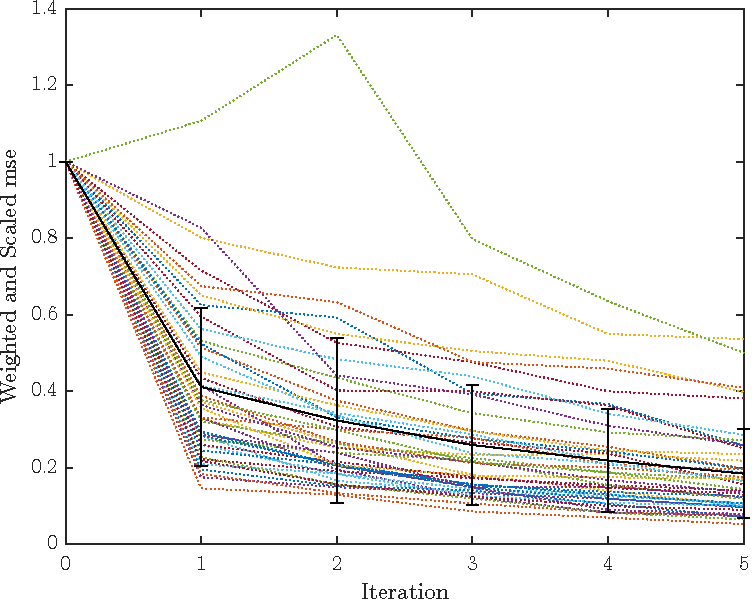
\includegraphics{dumb1.pdf}
        \caption[Monte Carlo]{Results of Monte Carlo sampling on the test datasets. Dotted lines represent the individual scoring for the data sets and the solid line shows the mean results at each iteration with error bars of $\frac{\sigma{}}{\sqrt{n-1}}$.}
        \label{fig:MCTestSet}
    \end{center}
\end{figure}

\subsection{Greedy}
Likewise, the Greedy algorithm was tested, with results presented in Figure~\ref{fig:GreedyTestSet}. Here, a final WMSE of ${0.323\pm{}0.039}$ was found indicating a worse scoring than the base case.
\begin{figure}[H]
    \begin{center}
        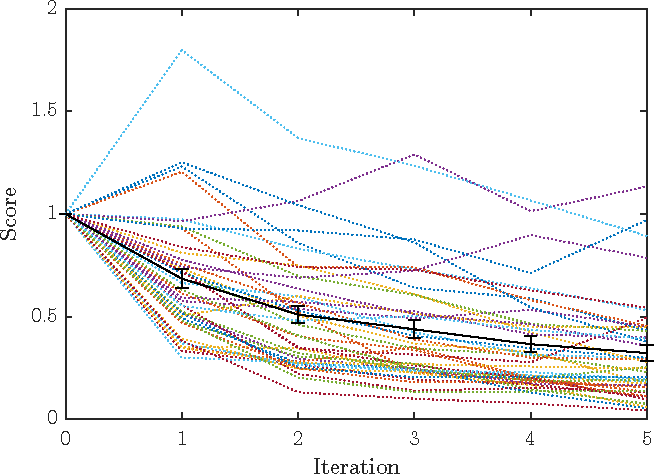
\includegraphics{greedy1.pdf}
        \caption[Greedy]{Results of greedy sampling on the test datasets. Dotted lines represent the individual scoring for the data sets and the solid line shows the mean results at each iteration.}
        \label{fig:GreedyTestSet}
    \end{center}
\end{figure}

\subsection{RoD Sampling}
The final non-parametic algorithm to be tested was RoD. A final WMSE of ${0.211\pm{}0.022}$, leading to a middling position between the other two parametric algorithms. The imporvement in each iteration is shown in Figure~\ref{fig:RODTestSet}.

\begin{figure}[H]
    \begin{center}
        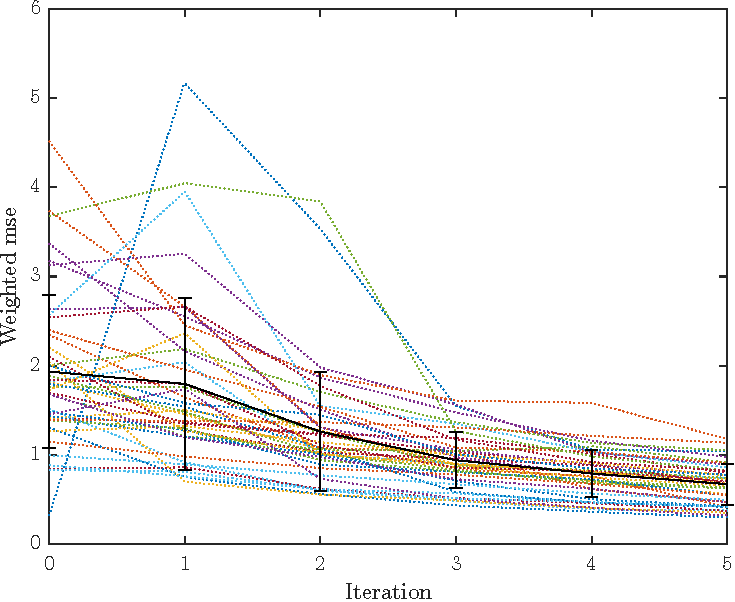
\includegraphics{rod1.pdf}
        \caption[RoD]{Results of RoD sampling on the test datasets. Dotted lines represent the individual scoring for the data sets and the solid line shows the mean results at each iteration.}
        \label{fig:RODTestSet}
    \end{center}
\end{figure}

\section{Parametric}
Parametric algorithms require a minimisation procedure on the training set. This leads to a computationally challenging script, and for this the author is grateful for the services provided by the HPC \cite{HPC}.

\subsection{Clusters}
The first set of algorithms tested were the clusters. Each of these outperformed all three of the other algorithms, with Cluster I, Cluster II, and Cluster III giving WMSEs of ${0.155\pm{}0.020}$, ${0.145\pm{}0.009}$, and respectively ${0.143\pm{}0.016}$. Due to the results from Cluster III, this is the one that will be used within the Holy Trinity. A variety of optimal ${c}$ were found when comparing to Algorithm~\ref{alg:cluster1}. An aditional cluster size of 45, 40, and 60 were found to be optimal for Cluster I, II, and III respectively.

\begin{figure}[H]
    \begin{center}
        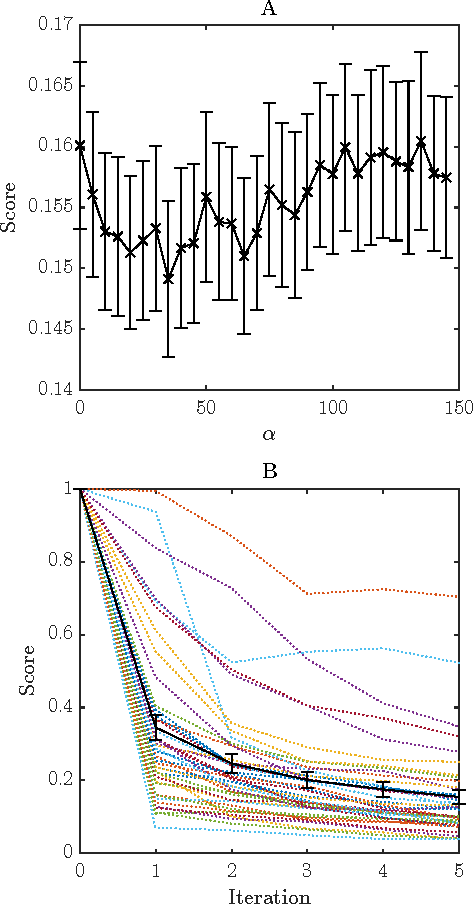
\includegraphics{cluster.pdf}
    \end{center}
\end{figure}
\begin{figure}[H]
    \begin{center}
        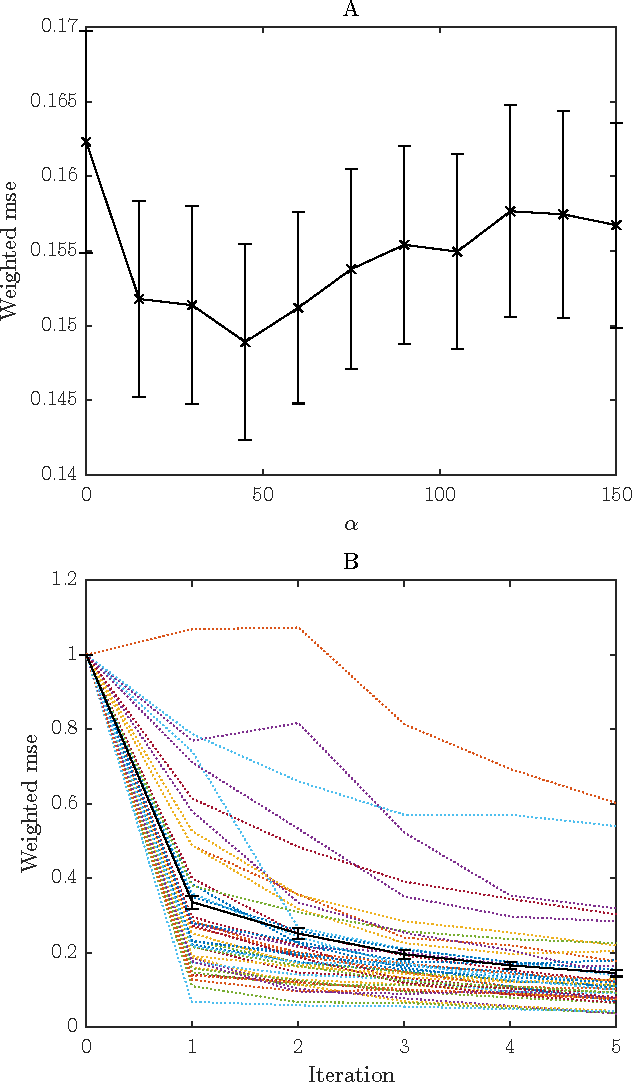
\includegraphics{clusterII.pdf}
    \end{center}
\end{figure}
\begin{figure}[H]
    \begin{center}
        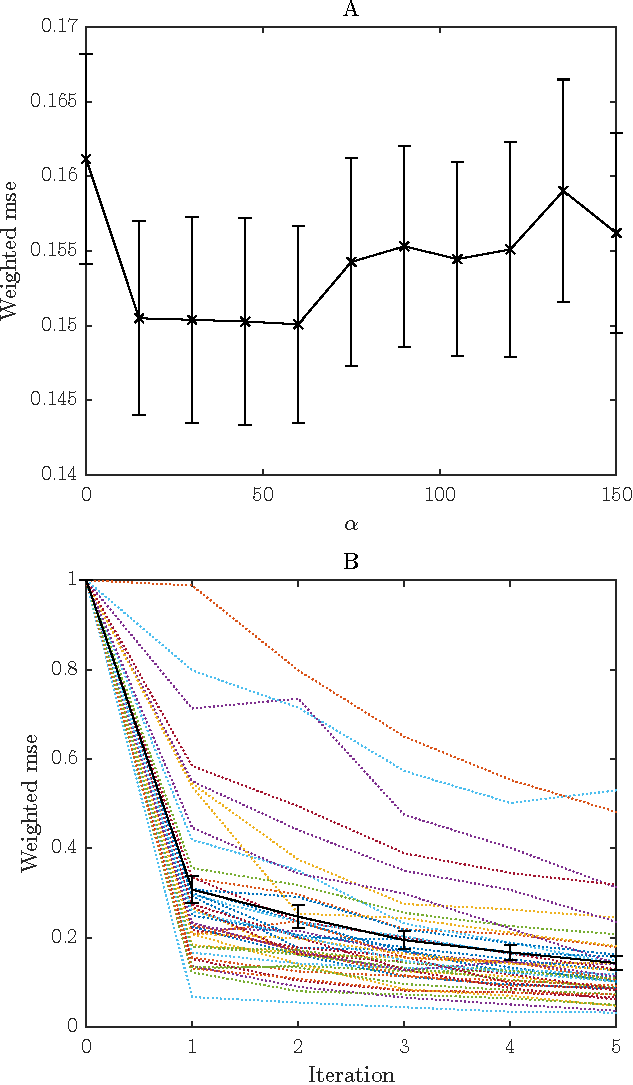
\includegraphics{clusterIII.pdf}
        \caption[Cluster III]{The results of fitting $c$ to the Cluster III algorithm. A) shows the results from parameter fitting and B) shows the learning process on the test set.}
        \label{fig:clusterTest}
    \end{center}
\end{figure}

\subsection{RoD with Greed}
When testing the RoD with greed sampling method, it was found that despite the weighting towards higher value targets, no improvement was seen over ROD with $\alpha{}=0.06$, with $\alpha$ defined in \ref{eq:rodAndGreed}. However, the tolerance at small $\alpha$, as shown in Figure~\ref{fig:rogreed}A. This mehtod gave a final a score of ${0.206\pm{}0.011}$, a slight improvement over simply using RoD.

\begin{figure}[H]
    \begin{center}
        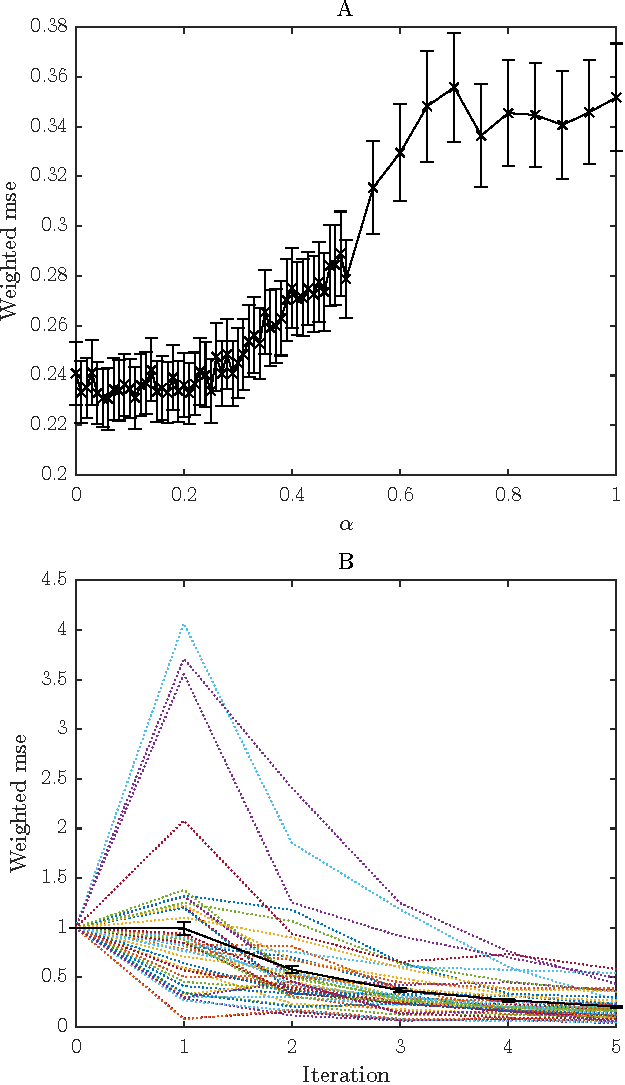
\includegraphics{rodGreedParam.pdf}
        \caption[RoD with Greed]{The results of fitting $\alpha{}$ to the RoD with Greed algorithm. A) shows the results from parameter fitting and B) shows the learning process on the test set.}
        \label{fig:rogreed}
    \end{center}
\end{figure}

\subsection{Holy Trinity}
By sampling multiple values for $\alpha$, a final set of $\alpha=[60, 0.4, 0.2]$ was reached where $[\alpha{}_1, \alpha{}_2, \alpha{}_3]$ correspond to the constants used in Algorithm~\ref{alg:cluster1}, \ref{eq:rodAndGreed}, and \ref{eq:holyTrinity} respectively. When validated against the testing datasets, a final result of $\mathrm{wmse}=0.116\pm{}0.014$ was found; the best result.

\begin{figure}[H]
    \begin{center}
        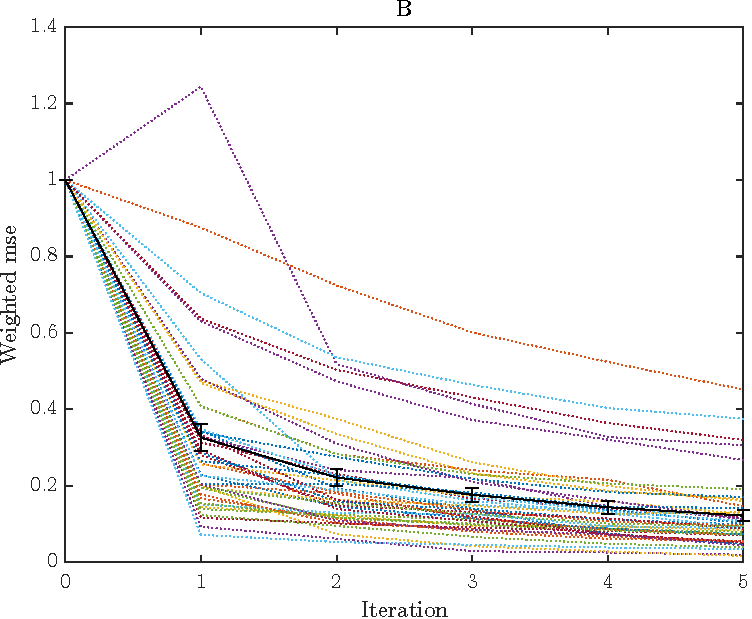
\includegraphics{holyGrail.pdf}
        \caption[Holy Trinity]{The results of fitting $\alpha{}$ to the Holy Trinity algorithm, showing the learning process on the test set. The learning of each data set has been added with dotted lines for illustative purposes.}
        \label{fig:holyTrinity}
    \end{center}
\end{figure}

% \section{Special Case: COVID-19}